%\begin{noindent}
\begin{markdown}

# Freileitungen

Sind elektrische Anlagen zur Übertragung elektrischer Energie

\GrayBox{Hochspannungsleitungen werden vorwiegend als Freileitungen gebaut, da diese günstiger als Erd- / Seekabel sind. \newline\newline Werden mit Dreiphasenwechselstrom betrieben, da dieser Vorteile bei der Transformierbarkeit mitbringen. Jedoch gibt es, bei großen Entfernungen, höhere Übertragungsverluste}

**Aufbau von Freileitungen**

- Masten
- Leiterseile (Oberirdisch verlegte Leitungen)
- Erdungen, Erdseil
- Isolatoren

**Forderungen von Freileitungen**

- Kurze und Geradlinige Leitungslängen
- Geringe Höhenunterschiede
- Geeignete Bodenverhältnisse für Masten und Erdung
- Wenig Kreuzungen mit anderen Leitungen, Eisenbahnen, Straßen, Flüsse und Bauwerke
- Vermeidung von Gebieten mit hoher Luftverschmutzung, explosionsgefährdeten Anlagen, Flugplätze und Sperrgebieten
- Geringer Eingriff in die Landschaft und Natur

## Arten von Masten

\end{markdown}

\begin{figure}[H]
    \centering
    \begin{subfigure}[t]{0.2\textwidth}
        \centering
        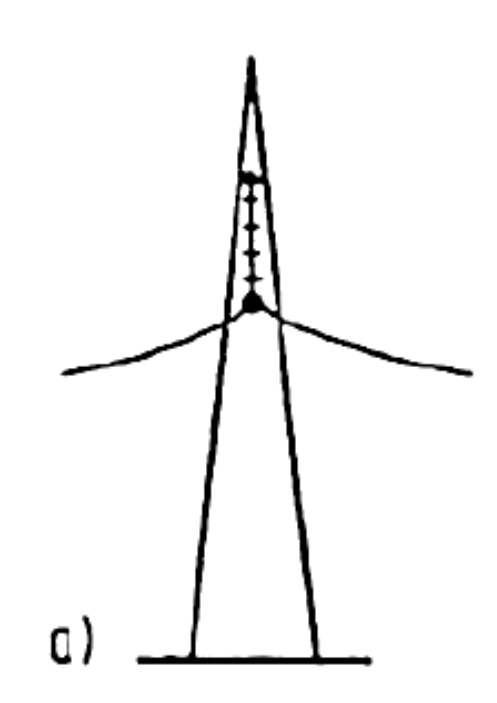
\includegraphics[height=3cm]{images/08-Freileitungen/Tragmast.png}
        \caption[Tragmast]{Tragmast (Reine Tragfunktion)}
    \end{subfigure}
    \hspace{1cm}
    \begin{subfigure}[t]{0.2\textheight}
        \centering
        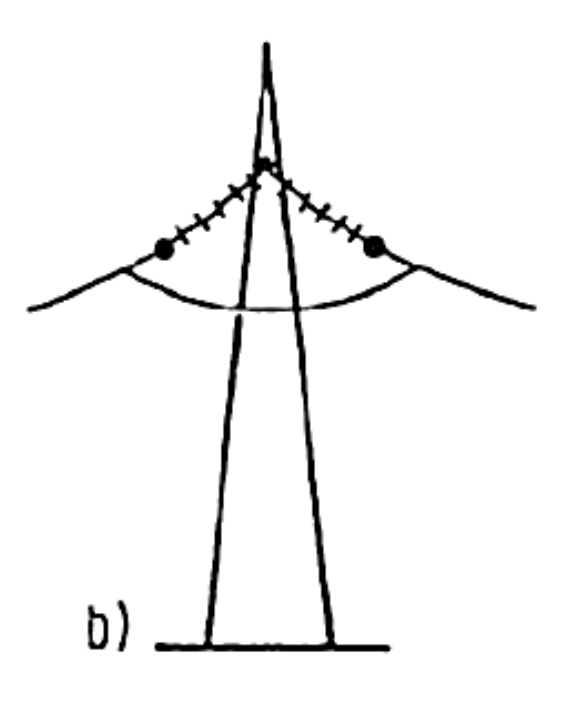
\includegraphics[height=3cm]{images/08-Freileitungen/Abspannmast.png}
        \caption[Abspannmast]{Abspannmast (Sektion von Leiterseil endet)}
    \end{subfigure}
    \hspace{1cm}
    \begin{subfigure}[t]{0.2\textwidth}
        \centering
        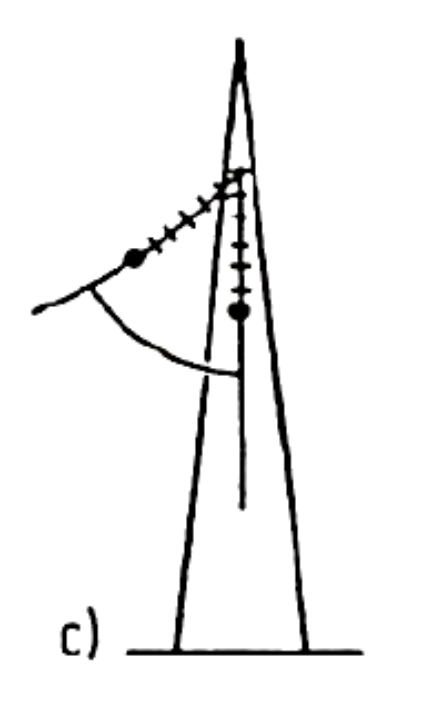
\includegraphics[height=3cm]{images/08-Freileitungen/Kabelendmasten.png}
        \caption[Kabelendmasten]{Kabelendmasten (Leitungsabzweigung / letzter Mast)}
    \end{subfigure}
    \caption[Arten von Masten]{Arten von Masten}
\end{figure}

%\begin{noindent}
\begin{markdown}

Bei Spannungen unter 110 kV werden meistens Holz-, Beton- und StahlgitterMasten verwendet, bei höheren Spannungen Stahlgittermasten)

## Eigenschaften von Leiterseile

- Meiste werden blanke Drähte und Seile als Leiter verwendet
- Einzeldrähte sind gegeneinander isoliert und werden verdrillt
- Bestehen aus Aluminium oder Aluminiumlegierungen
- Für eine mechanische Festigkeit wird z.B. ein Stahlkern benutzt
- Für große Leiterquerschnitte müssen die Stromdichten verringert werden

## Eigenschaften von Erdseile

- In der Seele befindet sich ein Stahlröhrchen mit eingezogenen Glasfasern zu Nachrichtenübertragung
- Wird bis zum Umspannwerk geführt und dort mit einem Erder verbunden
- Bei Netzfehlern (z.B. Kurzschluss zwischen Leiter und Mast) erfolgt eine Entlastung des Erdreiches und dadurch wird die Gefährdungsspannung geringer
- Leiterseile werden vor Blitzeinschlägen geschützt

## Korona Verluste (Sprühentladung)

\GrayBox{Können dazu führen, dass Leiter mit einem leuchtenden Kranz umgeben werden und bewirken Knistern und Funkstörungen}

\begin{itemize}
    \item[\textbf{Ursache}] Stark inhomogenes elektrisches Feld (hohe Feldstärke an der Leiteroberfläche, bei verhältnismäßig geringer Feldstärke im Raum)
\end{itemize}

Korona Verluste sind abhängig von Luftfeuchtigkeit, Temperatur und
Verschmutzung

**Um Korona-Verluste zu vermeiden, werden Bündelleiter eingesetzt.**

\vspace*{1em}

\begin{itemize}
    \item[\textbf{Bündelleiter}] Dabei wird ein Leiter auf mehrere parallele Teilleiterseile aufgeteilt (Vergrößerung der Oberfläche) und durch Abstandshalter (Spacer, Dämpfer) fixiert.
\end{itemize}

## Isolatoren

\GrayBox{Verbinden den Leiter mechanisch mit den Masten und trennen diese gleichzeitig galvanisch.}

**Forderungen von Isolatoren**

- Gutes Isoliervermögen _(auch bei ungünstigen Betriebsbedingungen – Regen, etc.)_
- Hohe mechanische Festigkeit _(bei wechselnder Belastung – Zugspannungen, etc.)_

Als Isolator-Material wird meist Glas oder Keramik verwendet.

\end{markdown}